\documentclass[10pt, a4paper]{article}
%-----------------------
%- 	PACKAGES & SETTINGS
%-----------------------
\usepackage[utf8]{inputenc}
\usepackage[italian]{babel}
\usepackage{xcolor}
\usepackage{hyperref}
\hypersetup{
    colorlinks=true,
    filecolor=magenta,      
    urlcolor=blue,
    linkcolor=black
}
\urlstyle{same}
\usepackage{amsmath}
\usepackage{graphicx}
\graphicspath{ {images/} }
 
%-----------------------
%- 	TITLE
%-----------------------
\title{\textbf{Relazione Progetto Java PR 2}}
\author{\textbf{Venturi} Ludovico\\Docente: \href{http://pages.di.unipi.it/levi/}{Francesca Levi}}
\date{UNIPI, Novembre 2019}


%-----------------------
%- 	DOCUMENT
%-----------------------
\begin{document}
%- 	INTRO
\pagenumbering{roman} 
\maketitle
\tableofcontents
\vfill
\begin{figure}[h]
	\centering
	
\includegraphics[scale=0.07]{javaLogo}
	\label{fig:0}
\end{figure}

\clearpage

%- 	START DOC
\pagenumbering{arabic} 
\section{Scelte progettuali}
Nella relazione verranno spiegate le scelte di implementazione e progettuali che sono state prese.

\subsection{Data}
\begin{center}
OVERVIEW: \textit{Data rappresenta un dato sottoforma di un insieme di 3 attributi e alcune operazioni. È una struttura astratta immutable, di dimensione finita e fissa.}
\end{center}
\textit{Data} viene implementata come classe astratta.
Tale scelta deriva dalla volontà di attribuire a tutte le classi che discendono da \textit{Data} delle caratteristiche comuni, ovvero dei metodi già implementati e una struttura implementativa di base:
\begin{center}
	\textit{private String \textbf{dataName};\\
	private String \textbf{content};\\
	private String \textbf{category};\\}
\end{center}
Come da specifica la classe \textit{Data} riporta anche il metodo astratto display che verrà implementato dalle sottoclassi.
\begin{center}
	\textit{public abstract void display();}
\end{center}
\textit{Data} ridefinisce anche \textit{equals()} per permettere la deep equality e mette a disposizione dei getter per accedere ai dati privati in lettura.\\
Rappresenta un \textit{contratto} cui tutte le sottoclassi (= i vari dati) dovranno sottostare, ovvero condivideranno con \textit{Data} la struttura di base, i vari metodi non astratti e dovranno ridefinire il metodo \textit{display()}.
\subsubsection{Ipotesi}
\begin{itemize}
 \item Non ci sono setter poichè si è ipotizzato che \textit{Data} fosse una struttura \textit{immutable}.
 \end{itemize}
 
\begin{footnotesize}
(setCategory() viene chiamato soltanto da )\\
(Nel testo viene riportato «\textit{i dati possono essere
visualizzati dagli amici ma modificati solamente dal proprietario della bacheca}»: ciò è stato interpretato come: "la modifica consiste nell'aggiunta o la rimozione dei dati, non nella  modifica effettiva del contenuto dei dati").
\end{footnotesize}
\subsubsection{MyData}
\textit{MyData} è una sottoclasse di \textit{Data}. Implementa il metodo display{} senza aggiungere altro alla struttura della sopraclasse.
\clearpage
\subsection{Board «E extends Data» }
\subsubsection{Ipotesi}
\begin{itemize}
\item Non sono ammessi elementi \textit{null}
\item Non sono ammessi duplicati di alcun genere
\end{itemize}

\subsubsection{Implementazione 1}
\begin{figure}[h!]
	\centering
	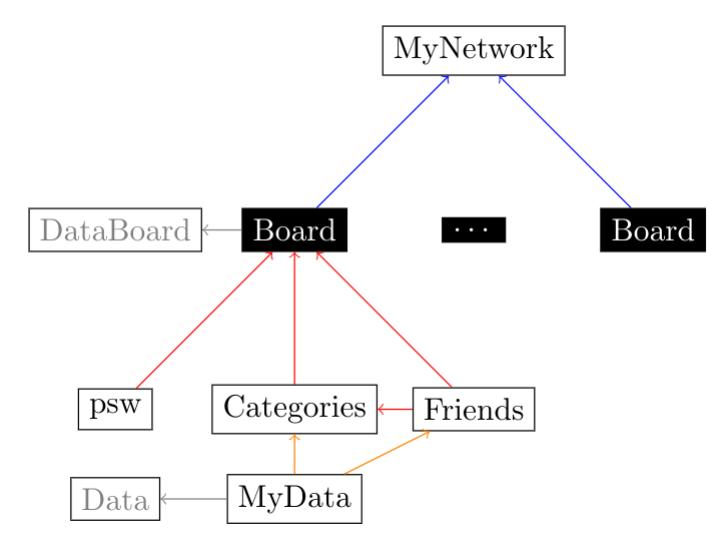
\includegraphics[scale=0.4]{diag1}
	\label{fig:diag1}
	\caption{Struttura generale del progetto con la prima implementazione di Board}
\end{figure}

Non ho riportato la specifica di ogni metodo nel codice di \textit{Board«E extends Data»} poichè risultava troppo confusionario; l'implementazione ha comunque seguito di pari passo la specifica riportata nell'interfaccia \textit{DataBoard«E extends Data»}.

\subsection{Implementazione 2: Board «E extends Data» }



\clearpage
\section{Eseguire il codice}
\subsection{Test ed esempi}
Non saranno verificate \textit{tutte} i casi in cui parametri sono null per ovvie ragioni.\\
Lista di test effettuati nel \textit{main}:
\begin{itemize}
\item password della bacheca « 8 caratteri
\item get di una bacheca non presente
\item password errata
\item categoria già presente
\item rimozione di una categoria non presente
\item 
\end{itemize}
% \href{www.multiplayer.it}{MULTIPLAYER}
% figura \ref{fig:im2} \pageref{fig:im2}
 
%\begin{itemize}
%  \item The individual entries are indicated %with a black dot, a so-called bullet.
%  \item The text in the entries may be of any %length.
%\end{itemize}

%$\begin{enumerate}



%\begin{equation}
%E=mc^2
%\end{equation}
%\subsection{daie}
%\label{sec:daie1}
%$ E=mc^2 $
%$\Omega + 3 = 54$\\
%$\omega * 54$

%\ref{table:tab1} SEZIONE \ref{sec:daie1}

%h = here
%\begin{table}[h]
%\centering
%\begin{tabular}{|c|c|r|}
%	\hline
%		cell1 & gatto & gattini \\
%	\hline
%		cell1 & gatto & 12 \\
%	\hline
%		cell1 & gatto & gattini \\
%	\hline
%\end{tabular}
%\label{table:tab1}
%\end{table}


\end{document}
